% !TEX root = ../main.tex
\newpage
\section{\mywork Emerging Network Topologies}
\subsection{\STDP applied to networks of theta neurons}
\textcolor{red}{TODO}: \textsl{explain in detail how the different methods \cref{eq:KempterSTDPFormulation2,eq:SongSTDPFormulation} will be implemented, using \STDP coupled with \IP.}

\begin{figure}[H]
\centering
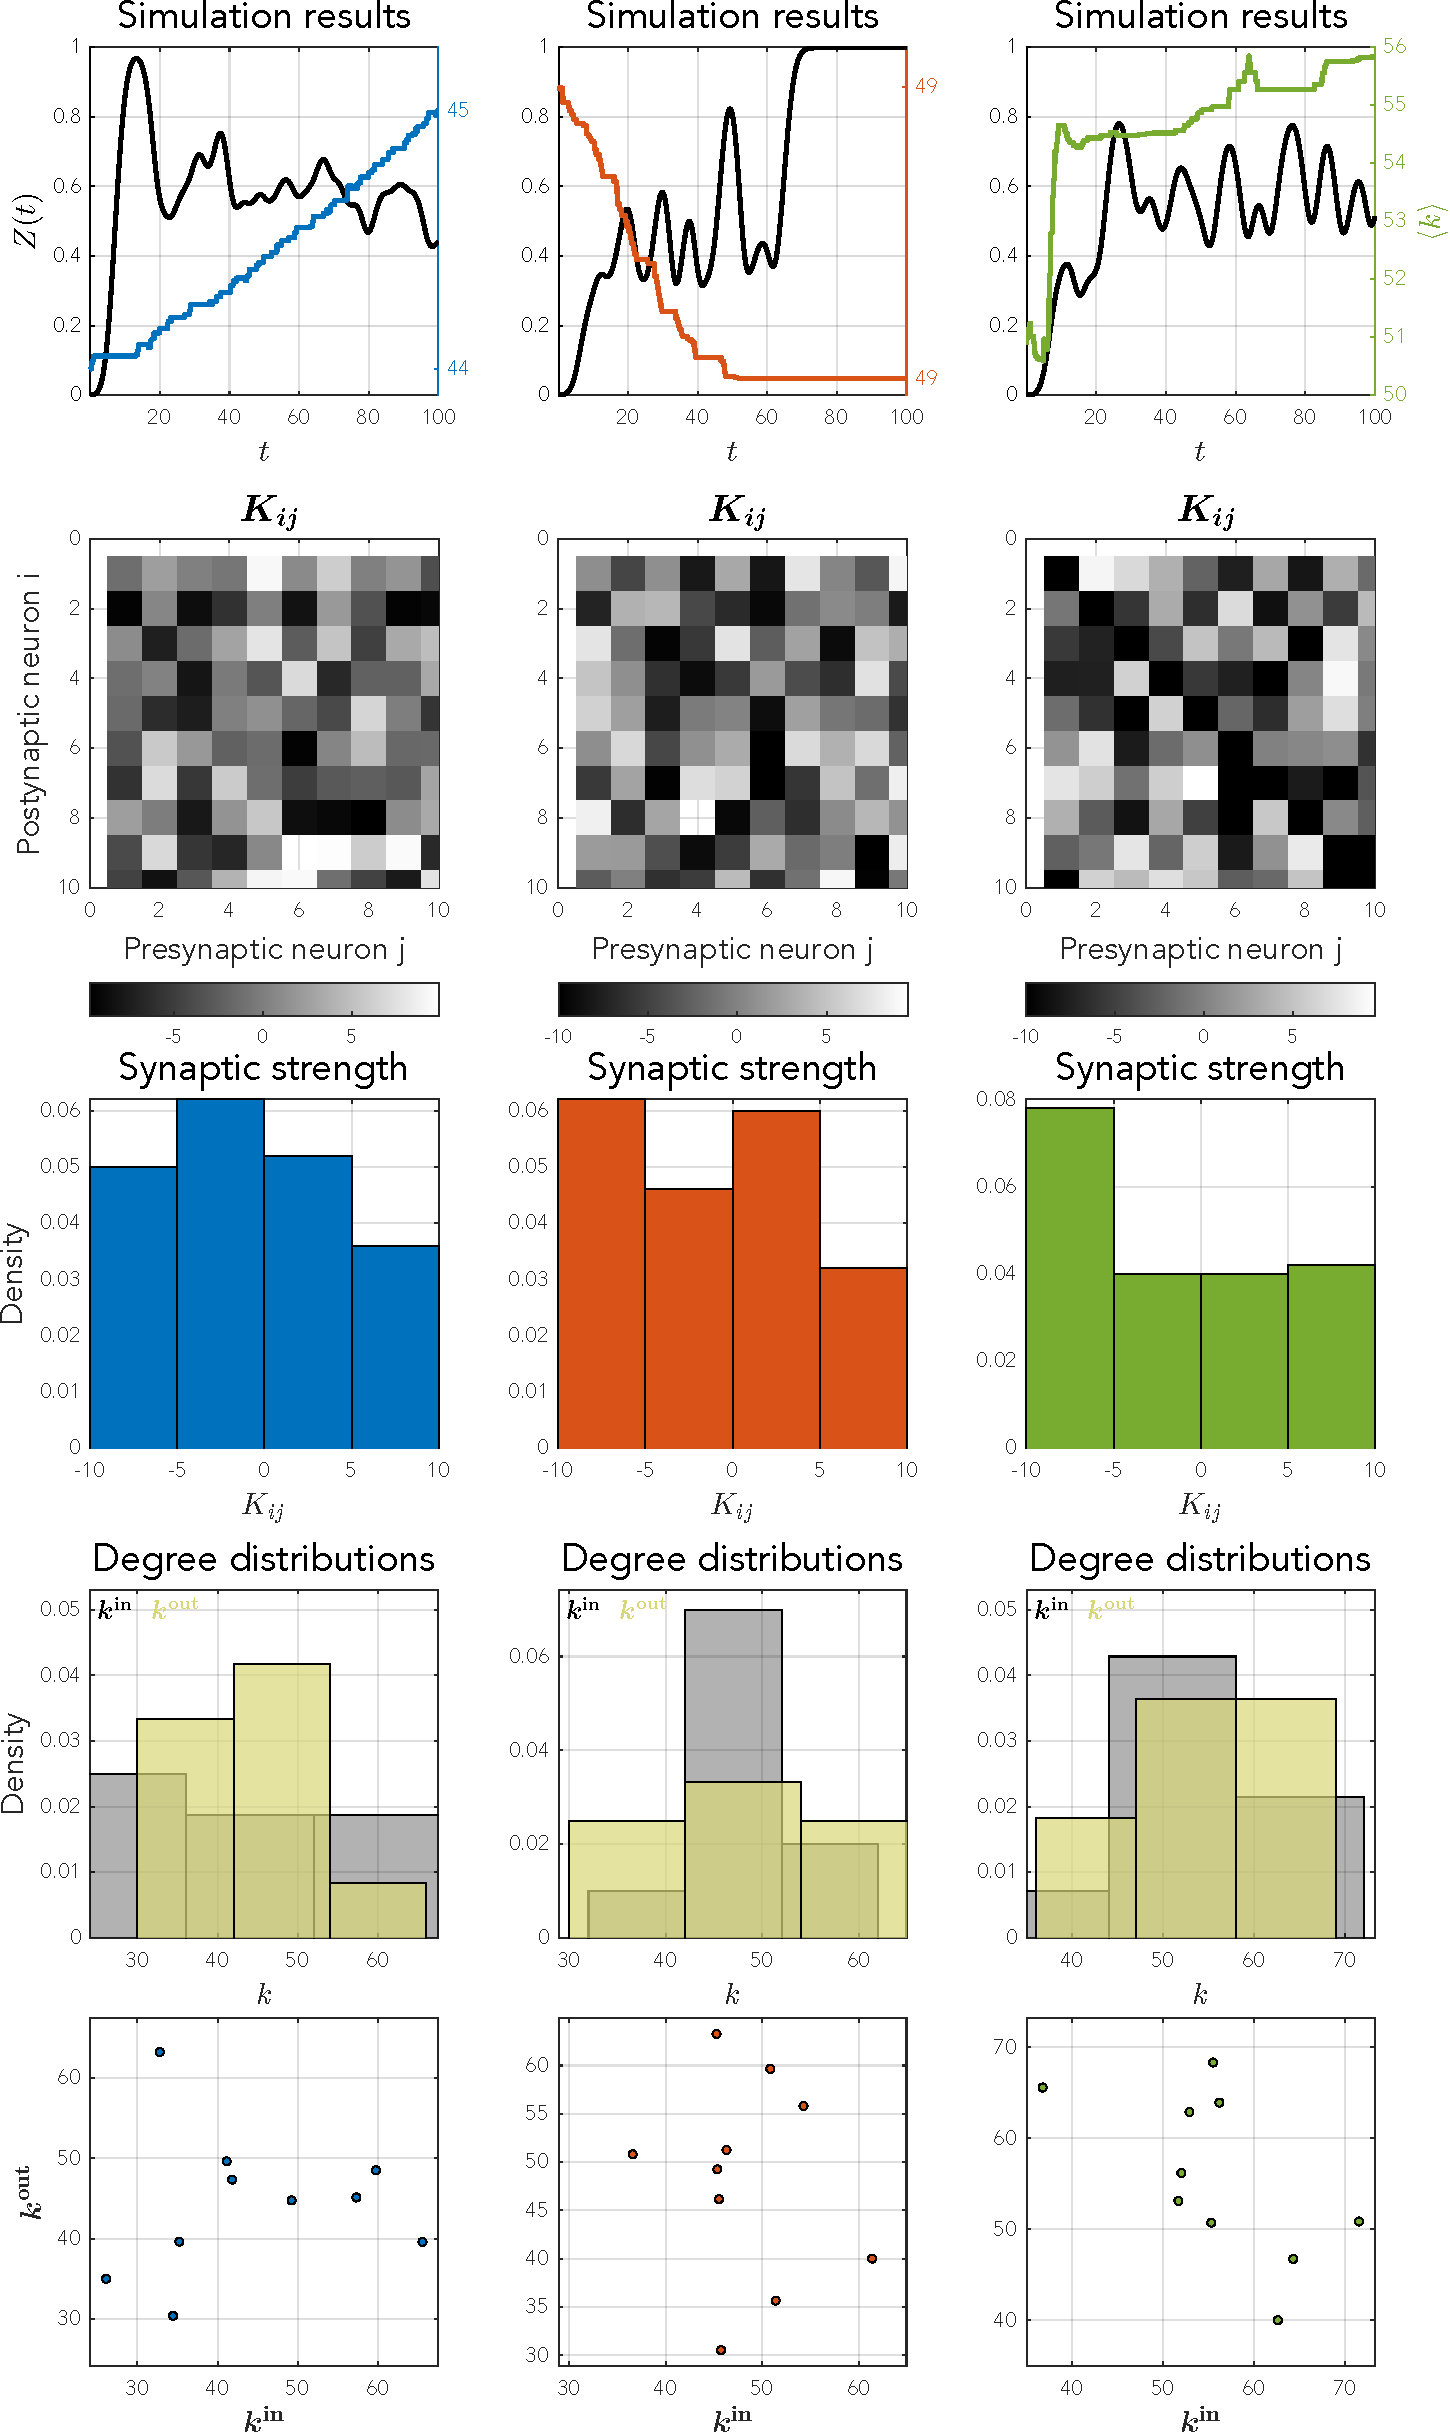
\includegraphics[height = \textheight]{../Figures/Learning/STDP.pdf}
\caption{Results of the \STDP learning.}
\label{fig:STDP}
\end{figure}

\begin{figure}[H]
\centering
\includegraphics[height = \textheight]{../Figures/Learning/STDPandIP.pdf}
\caption{Results of the \STDP learning with \IP learning.}
\label{fig:STDP}
\end{figure}



\begin{figure}[H]
\centering
\begin{subfigure}[b]{0.32\linewidth}
   \centering
  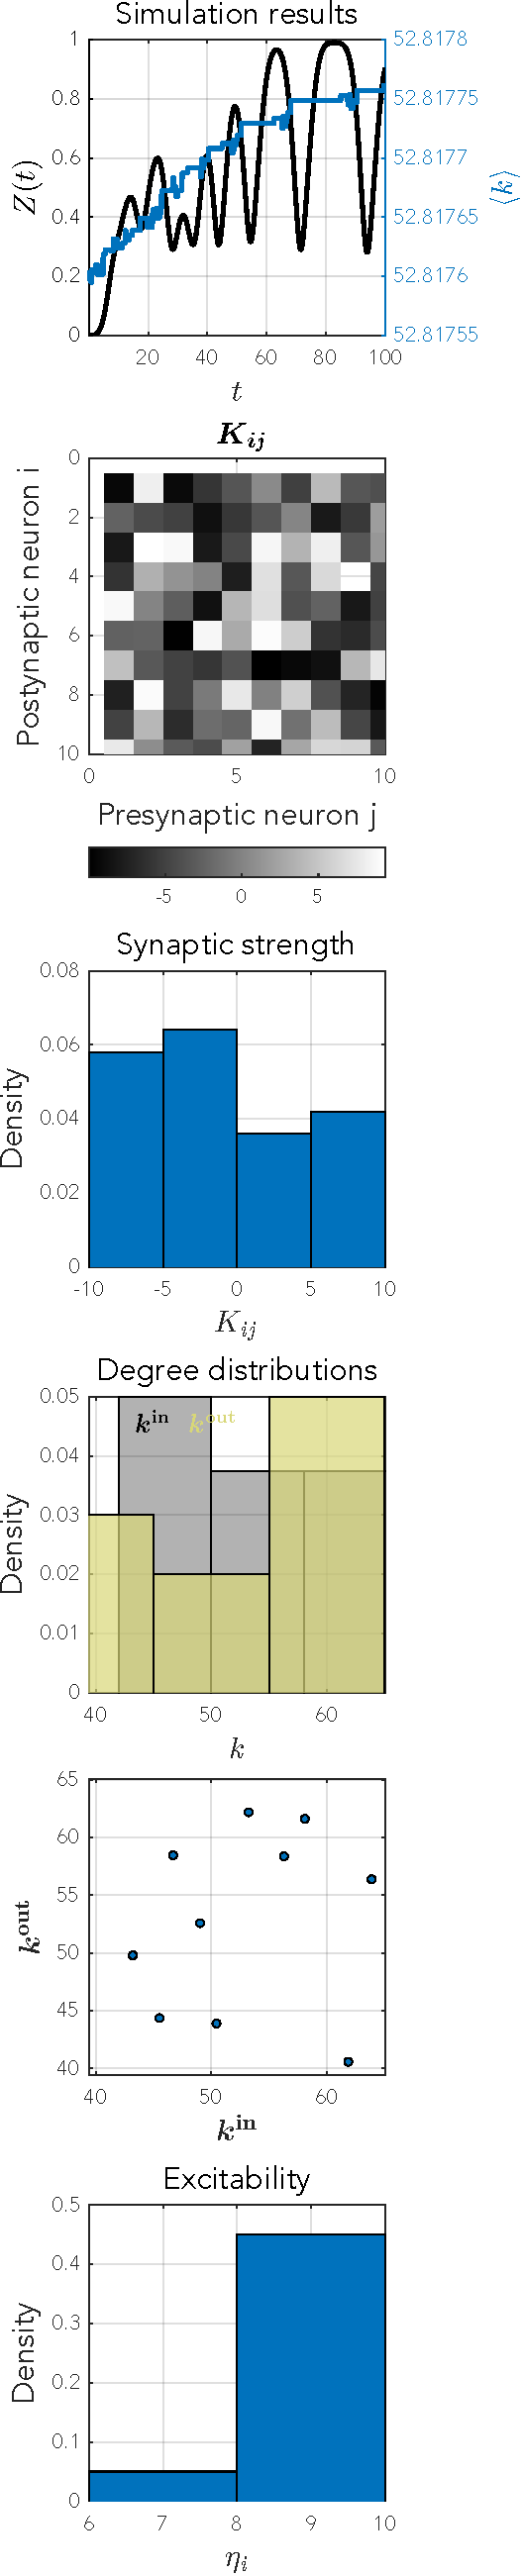
\includegraphics[width=\linewidth, trim={0 0 0 0 },clip]{../Figures/Learning/STDPandIPKempter.pdf}
   \caption{The window $W_K$.}
   \label{fig:STDPWK} 
\end{subfigure} \hfill
\begin{subfigure}[b]{0.32\linewidth}
   \centering
  \includegraphics[width=\linewidth, trim={0 0 0 0},clip]{../Figures/Learning/STDPandIPSong.pdf}
   \caption{The window $W_S$.}
   \label{fig:STDPWS}
\end{subfigure} \hfill
\begin{subfigure}[b]{0.32\linewidth}
   \centering
  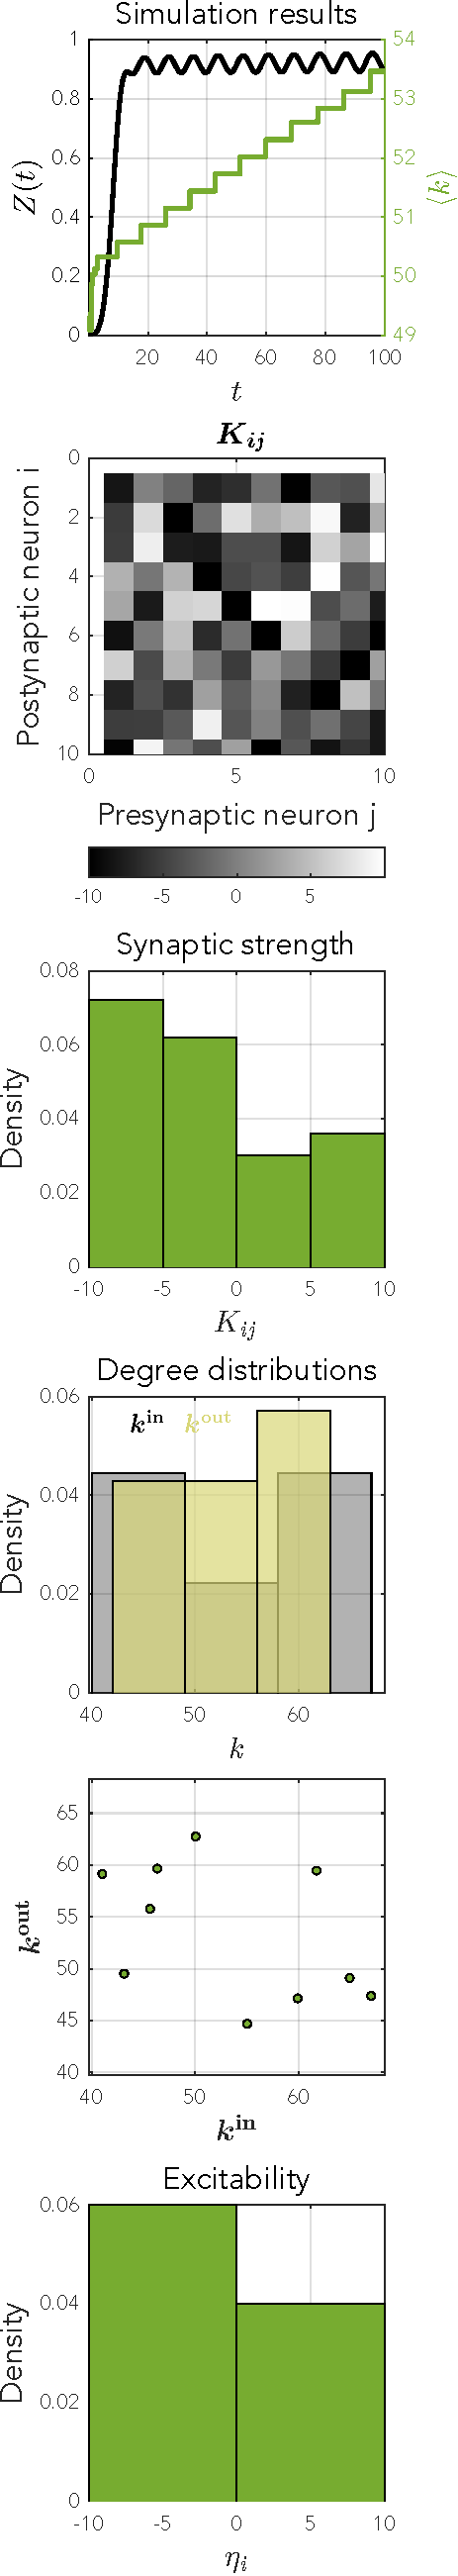
\includegraphics[width=\linewidth, trim={0 0 0 0},clip]{../Figures/Learning/STDPandIPChrolCannon.pdf}
   \caption{The window $W_C$.}
   \label{fig:STDPWC}
\end{subfigure}
   \caption{Results of the \STDP learning.}
   \label{fig:STDPresults}
\end{figure}



\subsection{Results}
\textcolor{red}{TODO}: \textsl{describe the emergent behaviour.}

